\section{The gradient of a scalar field}
\textcolor{red}{remove gradient from this and put this stuff later}
                        Related to the notion of partial differentiation and the gradient is that of finding the derivative of a function in a given direction.  Say that we are given a scalar field $f(x,y,z)$, and we are also given a unit vector $\unitvec$.  Then, we can compute the \boldgreen{directional derivative of $f$ in the direction $\unitvec$} by
                        \[
                        \frac{\partial f}{\partial \unitvec} = \unitvec \cdot \grad f.
                        \]
                        There is another way to define this derivative, but it requires a bit more work to derive.
                        
                                               
                        One can see that we can recover partial derivatives via this notion as well.  For example, if we let $\unitvec = \xhat$, then we have
                        \[
                        \frac{\partial f}{\partial \unitvec} = \xhat \cdot \grad f = \partialx.
                        \]
                        We can think of directional derivatives as generalizations of partial derivatives where we allow for computing the derivative of our function $f$ in a direction other than the ones given by the chosen basis.
                        
                        It turns out that collecting the partial derivatives as a vector is the best linear approximation to a scalar function.  We call this vector the gradient vector.
                        
                        \begin{df}{The Gradient}{gradient}
                        Given a scalar field $f(x,y,z)$, the \boldgreen{gradient of $f$ at the point $(x_0,y_0,z_0)$}, denoted $\grad f(x_0,y_0,z_0)$ is given by
                        \[
                        \grad f(x_0,y_0,z_0)=\begin{pmatrix} \partialx(x_0,y_0,z_0)\\ \partialy(x_0,y_0,z_0)\\ \partialz(x_0,y_0,z_0)\end{pmatrix}.
                        \]
                        \end{df}
                        
                        In fact, we often will consider the gradient as a vector itself.  That is, we will put
                        \[
                        \grad = \begin{pmatrix} \partialwrt{x} \\ \partialwrt{y} \\ \partialwrt{z} \end{pmatrix}.
                        \]
                        This will allow us to compute derivatives of vector fields by use of the cross and dot products.
                        
                        \begin{exercise}
                        Compute the gradient for the function
                        \[
                        f(x,y,z)=\sin(xyz)+x+2y^2+3x^2z.
                        \]
                        \end{exercise}

\textcolor{red}{Gradient properties}
                        \noindent\textbf{The Gradient:}
                        \begin{enumerate}[(i)]
                            \item \textbf{Sum Rule:} Given $f(x,y,z)$ and $g(x,y,z)$, we have that
                            \[
                            \grad(f(x,y,z)+g(x,y,z))=\grad f(x,y,z)+\grad g(x,y,z).
                            \]
                            \item \textbf{Constant Multiple:} Given $\lambda \in \R$ and $f(x,y,z)$, we have that
                            \[
                            \grad(\lambda f(x,y,z))=\lambda \grad f(x,y,z).
                            \]
                            \item \textbf{Product Rule:} Given $f(x,y,z)$ and $g(x,y,z)$ we have that
                            \[
                            \grad(f(x,y,z)g(x,y,z))=(\grad f(x,y,z))g(x,y,z)+f(x,y,z)(\grad g(x,y,z))
                            \]
                            
                        \end{enumerate}

                        We can put these together into the gradient $\nabla f$ and know how $f$ changes in each possible direction. Let's see how the gradient acts then. 
                        
                        \begin{ex}{Gradients on the Paraboloid}{gradients_paraboloid}
                        Let us start with $f(x,y)=x^2+y^2$.  Then
                        \[
                        \nabla f(x,y) = (2x,2y).
                        \]
                        Let us plot the level curves of this surface.
                        \begin{figure}[H]
                            \centering
                            \begin{subfigure}[h]{.45\textwidth}
                            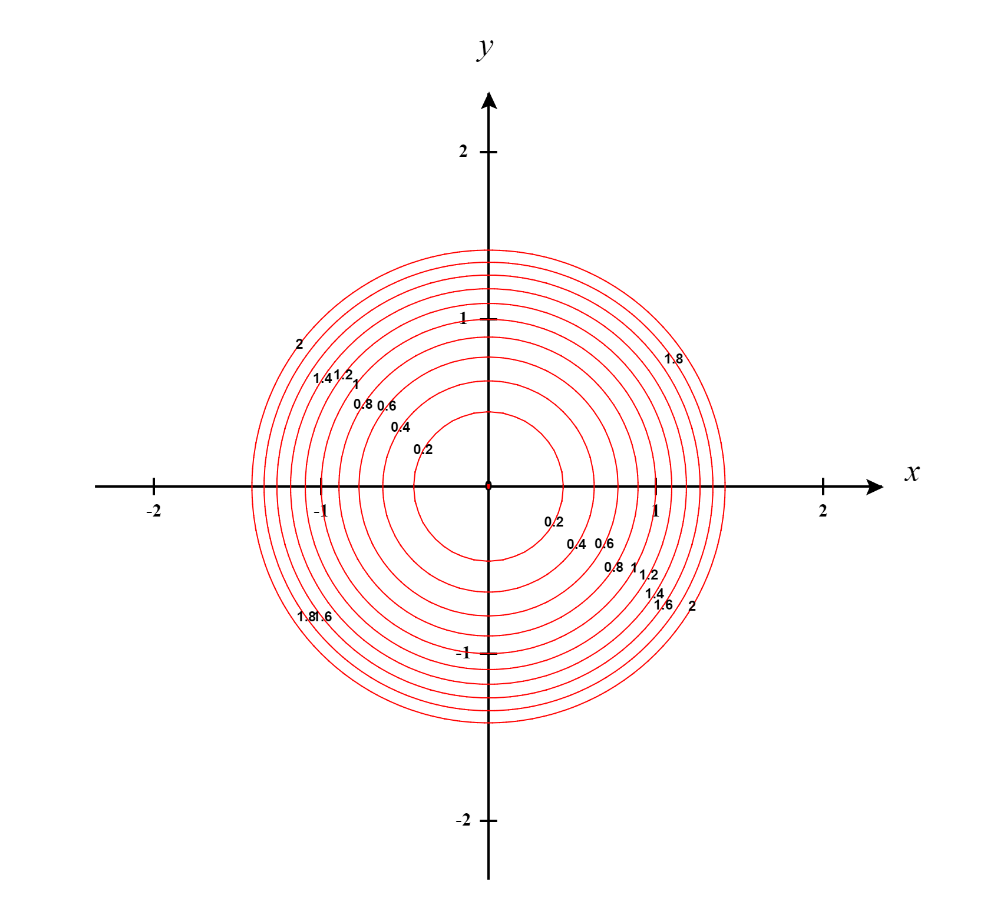
\includegraphics[width=\textwidth]{Figures_Part_6/level_curves_gradient.png}
                            \caption{Level curves of $f(x,y)$.}
                            \end{subfigure}
                            ~
                            \begin{subfigure}[h]{.45\textwidth}
                            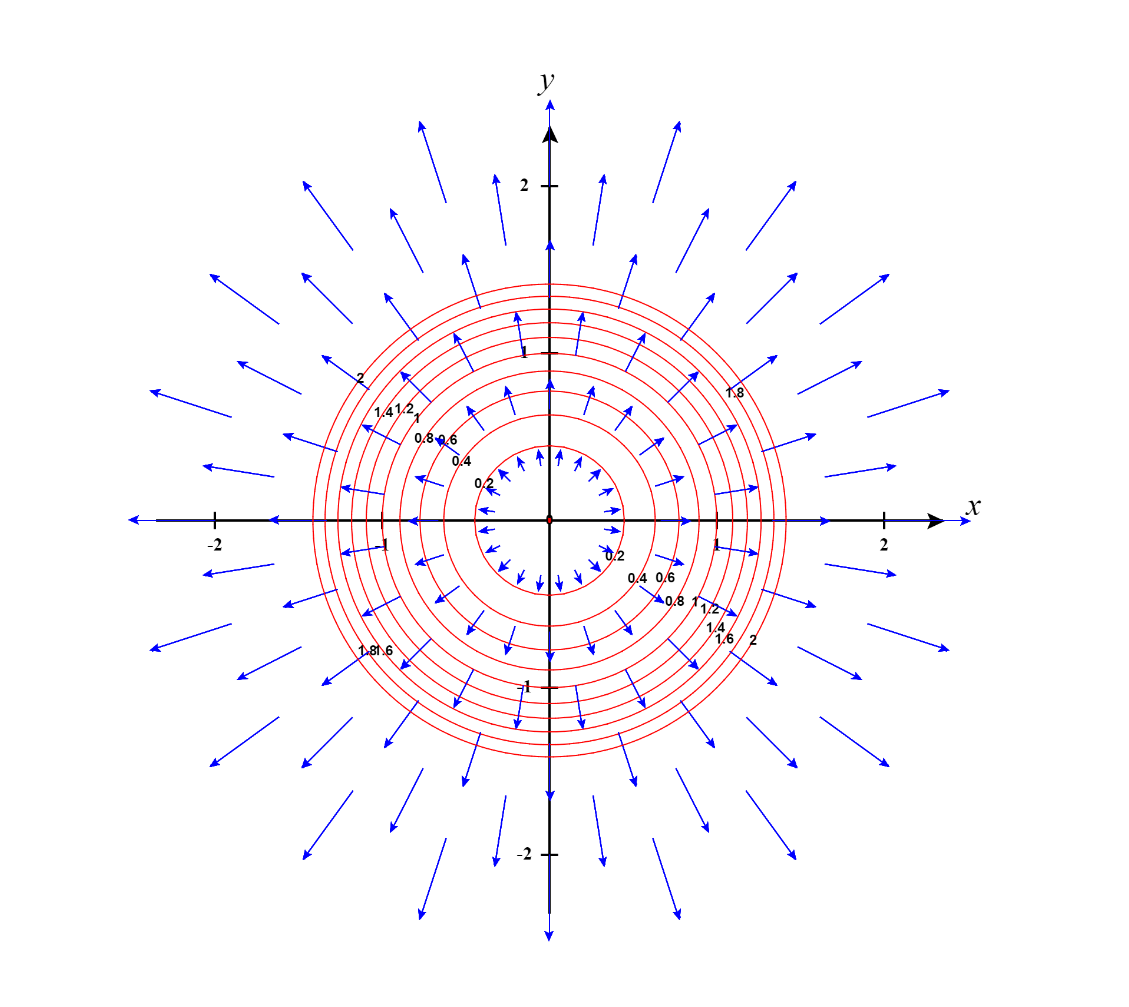
\includegraphics[width=\textwidth]{Figures_Part_6/level_curves_gradient_vectors.png}
                            \caption{Gradient vectors shown in blue.}
                            \end{subfigure}
                        \end{figure}
                        \begin{itemize}
                            \item Notice that the gradient vectors point in a direction perpendicular to the level curves and the length corresponds to how close the nearest level curve is.
                            \item The gradient is zero at the bottom of this surface.  
                        \end{itemize}
                        \end{ex}
                        
                        \begin{prop}{Gradient Points Uphill}{gradient_prop}
                        The gradient $\nabla f(x,y,z)$ is the vector that points in the direction of greatest increase for a function $f(x,y,z)$.
                        \end{prop}

\subsection{Optimization}
                        In single variable calculus, we optimized functions $f(x)$ by finding the point $x_0$ where 
                        \[
                        f'(x_0)=0.
                        \]
                        We called this a \emph{critical point}. We found if this optimizer $x_0$ was a maximizer or minimizer by checking the sign of second derivative $f''(x_0)$. We had
                        \begin{align*}
                            \textrm{Maximum: }& f''(x_0)<0\\
                            \textrm{Minimum: }& f''(x_0)>0.
                        \end{align*}
                        
                        In higher dimensions, this idea works similarly. We just have more to check. 
                        
                        \begin{df}{Stationary Points}{stationary_points}
                        Given a function $f(x,y)$, we call a point $(x_0,y_0)$ a \textbf{stationary point} if 
                        \[
                        \nabla f(x_0,y_0) = \mathbf{0}.
                        \]
                        \end{df}
                        
                        As before, we will use second derivatives to find out whether this is a maximum or a minimum.
                        
                        \begin{prop}{Maximizers and Minimizers}{max_min}
                        A stationary point $(x_0,y_0)$ is a 
                        \begin{align*}
                            \textrm{Maximizer if~ }& \frac{\partial^2 f}{\partial x^2} <0 \textrm{ ~and~ } \frac{\partial^2 f}{\partial y^2}<0,\\
                            \textrm{Minimizer if~ }& \frac{\partial^2 f}{\partial x^2} >0 \textrm{ ~and~ } \frac{\partial^2 f}{\partial y^2}>0,\\
                            \textrm{Saddle if otherwise.}
                        \end{align*}
                        \end{prop}
                        
                        \begin{exercise}
                        Let
                        \[
                        f(x,y) = \frac{xy}{e^{x^2+y^2}}.
                        \]
                        \begin{enumerate}[(a)]
                            \item Find all stationary points for $f$.
                            \item Determine whether these points are minimizers or maximizers.
                        \end{enumerate}
                        \end{exercise}
                        
                        \begin{exercise}
                        Show that $f(x,y)=xy$ has a saddle point at $(0,0)$.
                        \end{exercise}
                        
                        Some optimization problems cannot be solved just using this technique.  If you are interested, consider reading about \boldgreen{Lagrange multipliers}.

\section{Differentiation of Vector fields}
        We have already seen how we can differentiate curves and scalar fields.  Combining these two notions should give us what we need as far as building a derivative of a vector field goes.  Recall, given a curve $\curvegamma$, that the derivative is the tangent vector
        \[
        \tangentgamma = \begin{pmatrix} \dot{\gamma}_1 \\ \dot{\gamma}_2 \\ \dot{\gamma}_3 \end{pmatrix}.
        \]
        Likewise, if we are given a scalar field $f$, then the derivative is the gradient vector
        \[
        \grad f = \begin{pmatrix} \partialx \\ \partialy \\ \partialz \end{pmatrix}.
        \]
        A vector field is essentially a combination of a curve and scalar field in that it is as if we built a curve from scalar fields.  To be precise, a vector field truly defines the tangent vector to many curves that depend on their spatial position.  Imagine that a vector field describes the wind that can blow a particle from point to point.
       
        
        \begin{remark}
        Though we have not explicitly stated this before, this may be the most important take-away for calculus.
        
        \emph{The derivative of a function at a point is the best linear approximation to the function.} 
        
        Based on this wording, it is intuitive to imagine derivatives as vectors or matrices. The type of matrix that we receive as a derivative depends on the type of function that we wish to differentiate.  
        \end{remark}

\subsection{The Jacobian of a vector field}
		        Take a 3-dimensional vector field $\vecfieldV(x,y,z)$ by
		        \[
		        \vecfieldV(x,y,z)=\begin{pmatrix} V_1(x,y,z) \\ V_2(x,y,z) \\ V_3(x,y,z)\end{pmatrix},
		        \]
		        where we call each $V_1$, $V_2$, and $V_3$ the component functions.  Notice that each component function is a scalar field!
		        
		        Since each component function is a scalar field, we know how to compute the derivative of each by computing the gradient.  This gives us a way to then talk about the derivative of the vector field as a whole
		        
		        \begin{df}{Jacobian}{jacobian}
		        The \boldgreen{Jacobian} of a vector field $\mathbf{v}(x,y,z)$ is a matrix
		        \[
		        [J](x,y,z)\coloneqq \begin{pmatrix} \grad V_1^T \\ \grad V_2^T \\ \grad v_3^T \end{pmatrix},
		        \]
		        where the gradients are transposed (the superscript $T$) so they are are written as row vectors and placed in a matrix. More specifically, we can write this matrix as 
		        \[
		        [J](x,y,z) = \begin{pmatrix} \frac{\partial v_1}{\partial x} & \frac{\partial v_1}{\partial y} & \frac{\partial v_1}{\partial z}\\ \frac{\partial v_2}{\partial x} & \frac{\partial v_2}{\partial y} & \frac{\partial v_2}{\partial z} \\ \frac{\partial v_3}{\partial x} & \frac{\partial v_3}{\partial y} & \frac{\partial v_3}{\partial z} \end{pmatrix}.
		        \]
		        \end{df}
		        
		        The Jacobian contains a lot of information. Intuitively, it tells us how each component of the vector field changes in each direction.  In fact, the Jacobian essentially contains all the possible 1st order differential information that we could ever use for a vector field.  It will also allow us to compute coordinate transformations and volumes!
		        

		        
		        \begin{ex}{Computing the Jacobian, 1}{computing_jacobian}
		        Let us consider the vector field
		        \[
		        \vecfieldV(x,y,z) = \begin{pmatrix} x^2+y^2 \\ z \\x+y+z\end{pmatrix}.
		        \]
		        Then we can write
		        \begin{align*}
		            V_1(x,y,z)&= x^2+y^2\\
		            V_2(x,y,z)&= z\\
		            V_3(x,y,z)&= x+y+z.
		        \end{align*}
		        So we compute the gradients of each
		        \begin{align*}
		            \grad V_1 &= \begin{pmatrix} 2x \\ 2y \\ 0 \end{pmatrix}\\
		            \grad V_2 &= \begin{pmatrix} 0 \\ 0 \\ 1 \end{pmatrix}\\
		            \grad V_3 &= \begin{pmatrix} 1 \\ 1 \\ 1 \end{pmatrix}.
		        \end{align*}
		        So then the Jacobian is
		        \[
		        [J](x,y,z) = \begin{pmatrix} 2x & 2y & 0 \\ 0 & 0 & 1\\ 1 & 1 & 1 \end{pmatrix}.
		        \]
		        \end{ex}
		        
		        		       	This also tells us how a generalized product rule should work in this case.  Recall that we can take a scalar field $f(x,y,z)$ and multiply it by a vector field $\vecfieldV(x,y,z)$ to get $f\vecfieldV$.  Then, the Jacobian of this field is given by
		        		       	\[
		        		       	[J](x,y,z) = \begin{pmatrix} \grad (fV_1)^T \\ \grad(fV_2)^T \\ \grad(fV_3)^T\end{pmatrix},
		        		       	\]
		        		       	where we can then use the product rule for the gradient to compute the above statement.
		        		       	
		        
		        A related and important quantity comes in the form of the determinant of the Jacobian.  We've previously talked about the determinant of a matrix as telling us the (signed) scaling of volume of a linear transformation.  That is, for example, if we have
		        \[
		        A = \begin{bmatrix} 2 & 0 & 0\\ 0 & 2 & 0\\ 0 & 0 & 2 \end{bmatrix}
		        \]
		        then $\det(A)=8$ and we say that volumes of parallelopipeds are increased by a factor of $8$ in this case.  
		        
		        When you are given a vector field, you can think of different regions of space being stretched differently.  This is why we have that the Jacobian is a matrix that depends on the position $(x,y,z)$.  In this case, the volumes that are being stretched are very very tiny parallelopipeds.  You can think of cubes with side lengths $dx$, $dy$, and $dz$. 
		        
		        \begin{ex}{Computing the Jacobian, 2}{jacobian_2}
		        We found that given
		        \[
		        \vecfieldV(x,y,z) = \begin{pmatrix} x^2+y^2 \\ z \\ x+y+z\end{pmatrix}
		        \]
		        that
		        \[
		        [J](x,y,z) = \begin{pmatrix} 2x & 2y & 0 \\ 0 & 0 & 1 \\ 1 & 1 & 1 \end{pmatrix}
		        \]
		        As we can see, this matrix depends on position.  Let's compute the determinant
		        \[
		        \det([J](x,y,z))=2(y-x). 
		        \]
		        Something weird seems to happen with $y=x$ as the determinant $|[J](x,y,z)|$ will be zero in this case. In that case, it seems as if the volume along the plane given by $y=x$ is contracted to zero.
		        \end{ex}
		        
		        \subsection{Divergence and Curl}
		        Often we do not need to use the whole Jacobian.  We will find it to be necessary for integration, however.  For analysis of vector fields, we often wish to break them into their smaller pieces.  Fundamentally, we can break vector fields into two parts:
		        \begin{itemize}
		            \item Sources and sinks,
		            \item Rotations.
		        \end{itemize}
		        
		        \subsubsection{Sources, Sinks, and Divergence Fields}
		        With some vector fields, we can make the analogy that some quantity (think air or water) is being added or removed from the system.  We call these \boldgreen{sources} and \boldgreen{sinks} respectively.  We want to quantify how much of some quantity is being added. This quantity is called the \emph{divergence}.
		        
		        Recall, we can write
		        \[
		        \grad = \begin{pmatrix} \frac{\partial}{\partial x} \\ \frac{\partial}{\partial y} \\ \frac{\partial}{\partial z} \end{pmatrix}.
		        \]
		        If we are also given a vector field
		        \[
		        \vecfieldV(x,y,z) = \begin{pmatrix} V_1(x,y,z) \\ V_2(x,y,z) \\ V_3(x,y,z) \end{pmatrix},
		        \]
		        we can compute the \boldgreen{divergence} of $\vecfieldV$ by
		        \[
		        \grad \cdot \vecfieldV(x,y,z) = \frac{\partial V_1}{\partial x} + \frac{\partial V_2}{\partial y} + \frac{\partial V_3}{\partial z}.
		        \]
		        Notice that this quantity is a scalar!  This scalar value, the divergence, tells us how much the vector field is diverging at a point $(x,y,z)$. In other words, it tells us how much of a quanitity is being added or removed there.  In short, the divergence is the dot product of the gradient operator $\grad$ with the vector field $\vecfieldV$.  We can also realize the divergence as the trace of the Jacobian $\tr([J])$.  
		        
		        \begin{ex}{Source Field}{source_field}
		        Consider
		        \[
		        \vecfieldV(x,y,z) = \begin{pmatrix} x \\ y \\ z \end{pmatrix}.
		        \]
		        Then the divergence is
		        \[
		        \grad \cdot \vecfieldV(x,y,z) = \frac{\partial V_1}{\partial x} + \frac{\partial V_2}{\partial y} + \frac{\partial V_3}{\partial z} = 1 + 1 + 1 = 3.
		        \]
		        We can think of a source of air being placed at each point that pumps in $3$ units of air per second, or specifically being pumped in at the origin. The vector field looks like:
		        \begin{figure}[H]
		            \centering
		            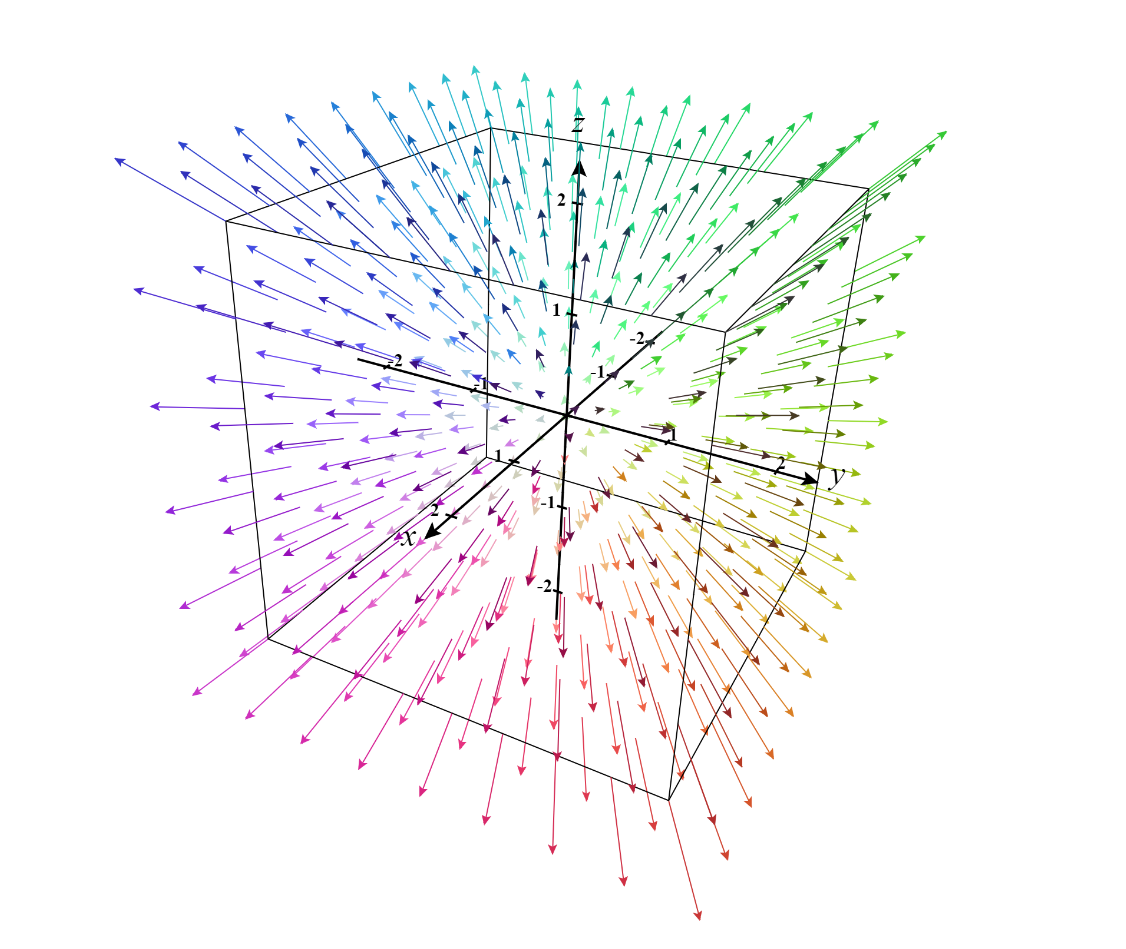
\includegraphics[width=.6\textwidth]{Figures_Part_6/divergence_field.png}
		        \end{figure}
		        Try to imagine that air is being pumped in from the origin, and the vector field shows the flow of the air out from the origin.
		        \end{ex}
		        
		        Say that we again take a scalar field $f(x,y,z)$ and multiply it by $\vecfieldV(x,y,z)$. How does this affect the divergence? Well, we can compute this using a more generalized notion of the product rule (or by realizing the divergence as the trace of the Jacobian via the earlier example).  We will find
		        \[
		        \grad \cdot (f\vecfieldV) = (\grad f)\cdot \vecfieldV + f (\grad \cdot \vecfieldV).
		        \]
		        
		        \begin{exercise}
		        Take any vector field and any scalar field and compute the above product rule.
		        \end{exercise}
		        
		        \subsubsection{Rotation Fields}
		        The divergence was the quantity that measured the outflow from a point for a vector field.  The other quantity we can measure is the \boldgreen{vorticity} of a vector field at a point. That is, how much a vector field looks like a ``vortex" around any given point.
		        
		        We define the \boldgreen{curl} of a vector field $\vecfieldV(x,y,z)$ to be
		        \[
		        \grad \times \vecfieldV(x,y,z) = \begin{pmatrix} \frac{\partial V_3}{\partial y} - \frac{\partial V_2}{\partial z} \\ \frac{\partial V_1}{\partial z} - \frac{\partial V_3}{\partial x} \\ \frac{\partial V_2}{\partial x} - \frac{\partial V_1}{\partial y} \end{pmatrix}.
		        \]
		        Note that the curl is a vector! The curl is a vector that points in a direction orthogonal to the plane where rotation in a field occurs and has magnitude relative to how quickly the field swirls. The direction of the curl also tells us whether the field rotates clockwise or counterclockwise in the plane of rotation as well.
		        
		        It's a bit involved to go through the work and see exactly why this is the correct quantity for seeing rotation of a vector field.  However, you can recall that the cross product was useful in describing rotational motion of rigid bodies (that is, it showed up in angular velocity/momentum).
		        
		        \begin{ex}{A Rotation Field}{rot_field}
		        Consider the vector field
		        \[
		        \vecfieldV(x,y,z) = \begin{pmatrix} -y \\ x \\ z\end{pmatrix}
		        \]
		        which looks like
		        \begin{figure}[H]
		            \centering
		            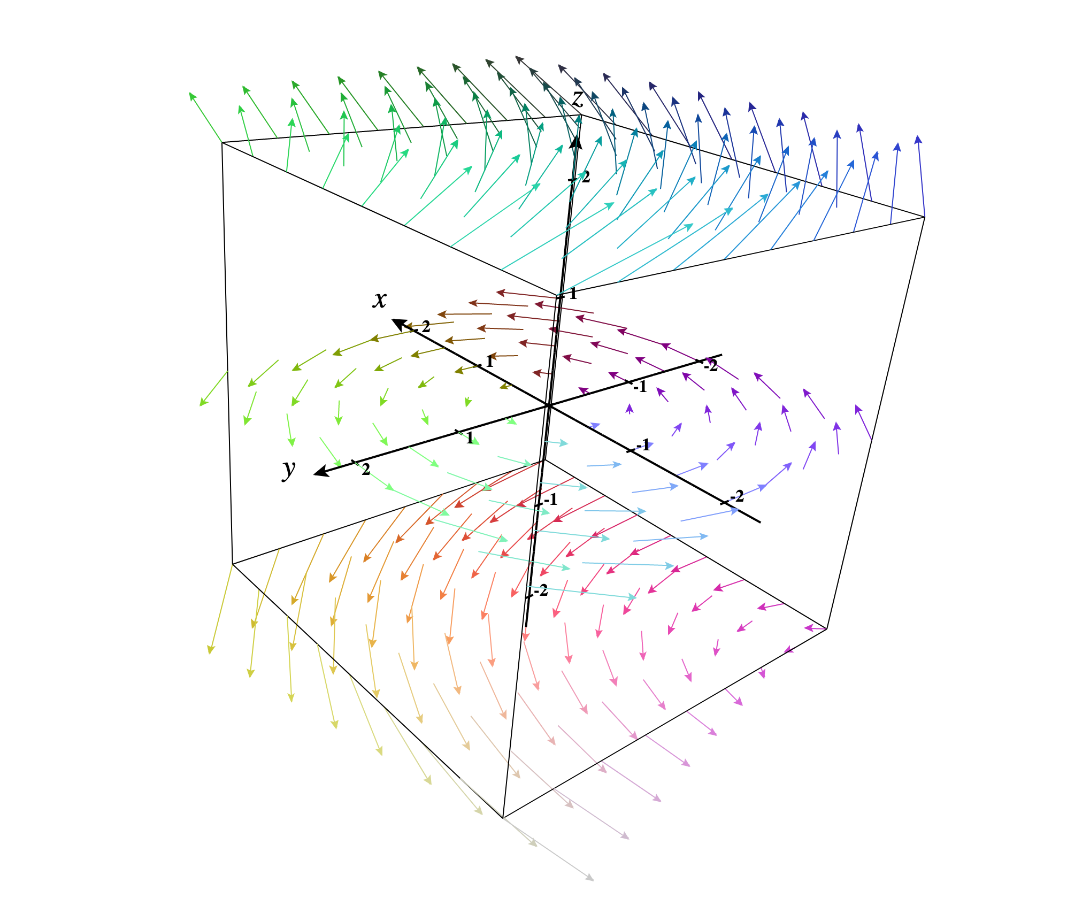
\includegraphics[width=.6\textwidth]{Figures_Part_6/curl_field.png}
		        \end{figure}
		        We let
		        \begin{align*}
		            V_1(x,y,z) &= -y\\
		            V_2(x,y,z) &= x\\
		            V_3(x,y,z) &= z.
		        \end{align*}
		        If we look in this figure where $z=0$, we can clearly see that this field swirls around the origin.  If the curl is to measure rotation, we should see it nonzero here.
		        
		        Let us compute the curl of this field.  For this, we will all the other partial derivatives not contained in the divergence. That is, we need
		        \begin{align*}
		            \frac{\partial V_1}{\partial y} &= -1 & \frac{\partial V_1}{\partial z} &= 0\\
		            \frac{\partial V_2}{\partial x} &= 1& \frac{\partial V_2}{\partial z} &= 0\\
		            \frac{\partial V_3}{\partial x} &= 0 &  \frac{\partial V_3}{\partial y} &=0.
		        \end{align*}
		        Then we have
		        \[
		        \grad \times \mathbf{v}(x,y,z) = \begin{pmatrix} 0-0\\ 0-0 \\ 1-(-1)\end{pmatrix} = \begin{pmatrix} 0\\ 0 \\ 2\end{pmatrix}.
		        \]
		        
		        We can decipher the meaning here by saying that the swirling occurs in planes parallel to the $xy$-plane since the direction of the curl is only in the $z$-direction.  That is, curl is pointing perpendicularly to the plane of rotation.  How quickly the field swirls is given by the magnitude of the curl which is $2$ in this case.  Using the right hand rule we discussed previously this tells us the direction of swirling as well.  We have swirling counter-clockwise in the planes parallel to the $xy$-plane, and so we expect the curl to point in the positive $z$-direction.
		    
		        \end{ex}
		        
		        \begin{exercise}
		        Plot the above field yourself and do a visual analysis of the vector field.
		        \end{exercise}
		        
		        \begin{ex}{Divergence of the Rotation Field}{div_of_rot_field}
		        One may also consider the divergent nature of the field 
		        \[
		        \vecfieldV(x,y,z) = \begin{pmatrix} -y \\ x \\ z\end{pmatrix}
		        \]
		        from the previous example and find that 
		        \[
		        \grad \cdot \vecfieldV(x,y,z) = 1.
		        \]
		        So, there is in some way divergence as well.  This leads us to breaking the vector field into a part that swirls and a part that diverges as follows:
		        \begin{align*}
		            \vecfieldV_\textrm{swirl}(x,y,z) &= \begin{pmatrix} -y \\ x \\ 0 \end{pmatrix}\\
		            \vecfieldV_\textrm{div}(x,y,z) &= \begin{pmatrix} 0 \\ 0 \\ z \end{pmatrix}.
		        \end{align*}
		        This type of analysis can be very helpful when considering real world problems.  It is especially important in electromagnetism.
		        \end{ex}
		        
		        \begin{remark}
		        	There is a general statement for the decomposition of vector fields given above.  It is known as the \boldgreen{Helmholtz decomposition}.  This decomposition is very important in the study of electromagnetism as it allows for one to fully decompose the symmetry group of the electromagnetic theory.
		        			        \end{remark}
		        			        
		       Once again, we may wonder how this can be affected if we multiply our vector field by a scalar field.  That is, how do we evaluate $\grad \times (f\vecfieldV)$?  Again, this comes from a more general product rule, and we have
		       \[
		       \grad \times (f \vecfieldV) = (\grad f)\times \vecfieldV + f (\grad \times \vecfieldV).
		       \]
		        
		        \subsubsection{Constant Vector Fields}
		        Most of the understanding of vector fields was just covered by understanding the the part that diverges and the part that curls.  However, you can always add constants to these vector fields and these constants will not change the divergence or curl. Why? Take the following example.
		        
		        \begin{ex}{Constant Fields}{const_field}
		        Let 
		        \[
		        \mathbf{v}(x,y,z) = (c_1,c_2,c_3)
		        \]
		        where $c_1,c_2,$ and $c_3$ are constants.  Then we can compute the Jacobian of $\mathbf{v}$
		        \[
		        J(x,y,z) = \begin{bmatrix} 0 & 0 & 0 \\ 0 & 0 & 0\\ 0 & 0 &0 \end{bmatrix}.
		        \]
		        Since the Jacobian holds all the partial derivative information, we can know from this that 
		        \begin{align*}
		            \nabla \cdot \mathbf{v} &= 0\\
		            \nabla \times \mathbf{v} &= \mathbf{0}.
		        \end{align*}
		        \end{ex}
		        
		        \begin{exercise}
		        Specifically show that the divergence and curl of a constant vector field (as in the previous example) are zero.  
		        \end{exercise}
		        
		        All of this is to say that aside from the addition of a constant vector field, we understand the behavior by looking at divergence and curl.      


       \section{Laplace Operator}
       
       Underlying the dynamics of many differential equations is an operator known as the \boldgreen{Laplacian} or \boldgreen{Laplace operator}.  There are many reasons why this operator is so special, but one fundamental reason is it describes the sums of curvatures at each point (at least with scalar functions).  In studying second order ODEs we came across the operator
       \[
       -\frac{d^2}{dx^2},
       \]
       which is the Laplace operator in one dimension. This operator described the curvature of a 1-dimensional rod. We will now seek to generalize this operator so that we may describe the curvature of a higher dimensional membrane.  We will also define an analogous operator for vector fields.
       
       Fundamentally, in physics, we take the belief that fields tend to be \emph{minimal} in some sense.  When it comes to scalar fields, we can imagine their graph, and find scalar fields that have minimal deformation energy given that the function must have certain boundary conditions. This is known as the minimal surface problem. This is where the scalar Laplace operator enters.  Likewise, to find minimal vector fields, we should have analogous notion, and we do.  If we were to place a number of sinks and sources in space, we could find the vector field that minimizes the energy of this configuration. This amounts to finding the solution to an equation involving the vector Laplacian.
       
        \subsection{The Laplacian of a Scalar Field}
               In the study of partial differential equations (PDEs), we are often asked to find a function $u(x,y,z)$ that satisfies the following equation
               \[
               \grad \cdot \grad u(x,y,z) = f(x,y,z)
               \]
               for some given function $f(x,y,z)$.  We will revisit this in the next part, but for now we should see exactly what we mean by
               \[
               \grad \cdot \grad u(x,y,z).
               \]
               
               \begin{exercise}
               Show that
               \[
               \grad \cdot \grad u(x,y,z) = \frac{\partial^2 u}{\partial x^2} + \frac{\partial^2 u}{\partial y^2} + \frac{\partial^2 u}{\partial z^2}.
               \]
               \end{exercise}
               
               \begin{df}{Laplacian}{laplacian}
               We define the quantity
               \[
               \grad \cdot \grad u(x,y,z)
               \]
               to be the \boldgreen{scalar Laplacian} of $u(x,y,z)$ and we often write
               \[
               \Delta \coloneqq \grad \cdot \grad.
               \]
              
               \end{df}
               
               Intuitively, the Laplacian can be summed up in a few ways. 
               \begin{itemize}
                   \item The Laplacian is the \emph{divergence} of the \emph{gradient} of a scalar function.
                   \item The Laplacian is the sum of ``curvatures" in each direction.
               \end{itemize}
               
               \begin{ex}{Computing the Laplacian}{compute_laplacian}
               Let us consider the functions
               \[
               f(x,y) = x^2+y^2
               \]
               and
               \[
               g(x,y) = x^2-y^2.
               \]
               Then we can compute the gradients of each function to get
               \begin{align*}
                   \grad f(x,y) &= \begin{bmatrix} 2x \\ 2y \end{bmatrix}\\
                   \grad g(x,y) &= \begin{bmatrix} 2x \\ -2y \end{bmatrix}.
               \end{align*}
               We can then compute the divergence of each of these and find
               \begin{align*}
                   \grad \cdot \grad f(x,y) &= 2+2 = 4\\
                   \grad \cdot \grad g(x,y) &= 2-2 =0.
               \end{align*}
               Let us see what these two functions look like to get a bit of an intuitive feel.
               \begin{figure}[H]
                   \centering
                   \begin{subfigure}[h]{.45\textwidth}
                   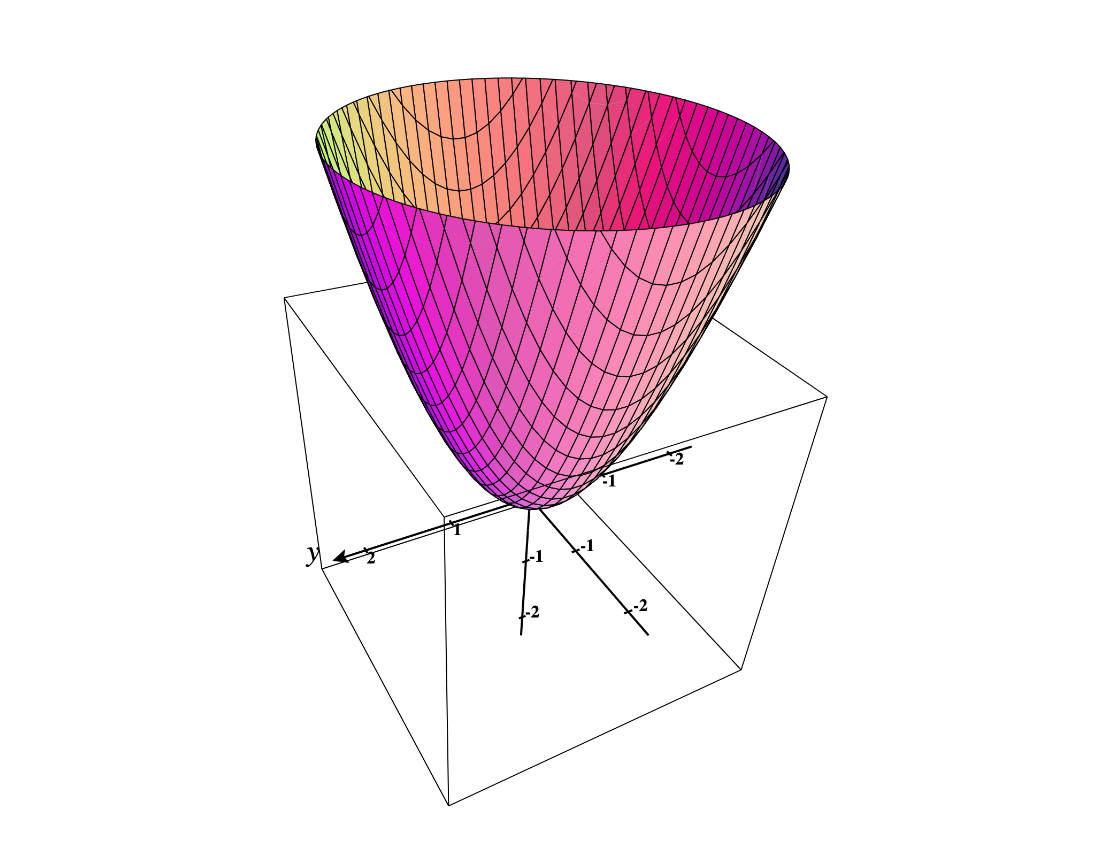
\includegraphics[width=\textwidth]{Figures_Part_6/pos_laplace.png}
                   \caption{A plot of $f(x,y).$}
                   \end{subfigure}
                   ~
                   \begin{subfigure}[h]{.45\textwidth}
                   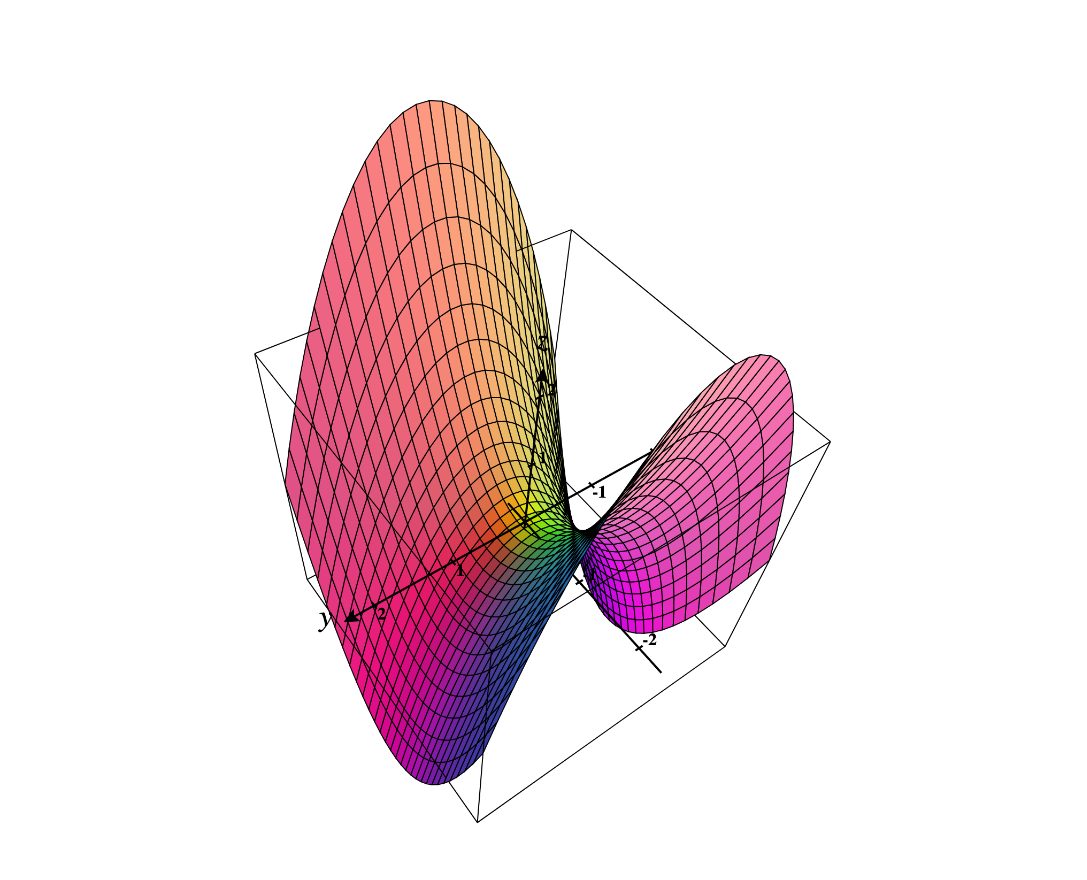
\includegraphics[width=\textwidth]{Figures_Part_6/0_laplace.png}
                   \caption{A plot of $g(x,y).$}
                   \end{subfigure}
               \end{figure}
               Fundamentally we can see that these two functions are different.  It seems that for $f(x,y)$ we are curving upward in both the $x$ and $y$ direction which is what allows the Laplacian to be positive. However, for $g(x,y)$ one direction curves the opposite direction as the other which cancels out and gives us that the Laplacian is zero.  
               
               It turns out that the Laplacian describes many phenomenon. Two examples would be soap films and temperature flow.
               \end{ex}
       
               
               \subsection{Vector Laplacian}
               
               As stated in the introduction to this section, there exists an analogous operator known as the \boldgreen{vector Laplacian}.  Given a vector field $\vecfieldV(x,y,z)$, we define the vector Laplacian by
               \[
               \veclaplace \vecfieldV \coloneqq \grad(\grad \cdot \vecfieldV)-\grad \times (\grad times \vecfieldV).
               \]
               In our cartesian coordinate system, we can write this as
               \[
               \veclaplace \vecfieldV = \begin{pmatrix} \Delta V_1 \\ \Delta V_2 \\ \Delta V_3 \end{pmatrix}.          
               \]
               Let us compute this with an example.  
               
               \begin{ex}{Electric Field}{electric_field_laplace}
               Say we place a point charge of 1 at the origin.  The electric field given by this point charge is then
               \[
               \vecfieldE(x,y,z) = \begin{pmatrix} \frac{-x}{\left(x^2+y^2+z^2\right)^{3/2}} \\ \frac{-y}{\left(x^2+y^2+z^2\right)^{3/2}} \\ \frac{-z}{\left(x^2+y^2+z^2\right)^{3/2}} \end{pmatrix}.
               \]
               Then, we can compute the vector Laplacian of this field
               \[
               \veclaplace \vecfieldE = \grad(\grad \cdot \vecfieldE) - \grad \times (\grad \times \vecfieldE).
               \]
               Note that we have $\grad \times \vecfieldE = 0$ (which is known as Faraday's law). Hence, we need only compute
               \[
               \veclaplace \vecfieldE = \grad(\grad\cdot \vecfieldE).
               \] 
               We have that
               \begin{align*}
               \grad \cdot \vecfieldE &= \frac{\partial V_1}{\partial x} +  \frac{\partial V_2}{\partial y} +  \frac{\partial V_3}{\partial z}\\
               &= \frac{-2x^2+y^2+z^2}{\left(x^2+y^2+z^2\right)^{5/2}} + \frac{x^2-2y^2+z^2}{\left(x^2+y^2+z^2\right)^{5/2}}+\frac{x^2+y^2-2z^2}{\left(x^2+y^2+z^2\right)^{5/2}}\\
               &= 0, \textrm{~ everywhere except at $(x,y,z)=0$}.
               \end{align*}
               Thus, it must be that
               \[
               \veclaplace \vecfieldE = 0, \textrm{~except for at the origin.}
               \]
                 This means that, in some sense, the electric field is the minimal field given this source configuration.  We will ignore the origin in this computation, but the solution is related to the delta function.  More on this later.
               \end{ex}
               
               \begin{exercise}
               Verify that the above computations are correct. Specifically, compute $\grad \times \vecfieldE$ and compute the vector Laplacian by taking the scalar Laplacian of each component.
               \end{exercise}
              
       
       \section{Composite Functions and Chain Rule}
       
       We have introduced curves $\curvegamma$, scalar fields $f$, and vector fields $\vecfieldV$ as the fundamental types of functions in the space $\R^3$.  Given these types of functions, we can also consider composite functions such as
       \[
       f\circ \curvegamma, \qquad \vecfieldV \circ \curvegamma, \qquad f \circ \vecfieldV.
       \]
     	We will work through each example, and realize the derivative of the composite functions as well. Hence, we are seeking to generalize the chain-rule from single variable calculus.
     	
     	Earlier, we briefly remarked that \emph{the derivative of a function is the best linear approximation to that function.} So, let us briefly revisit a few things.
     	
     	First, if we have a curve $\curvegamma \colon \R \to \R^3$, we computed the derivative of this curve as $\tangentgamma$. Keep in mind, we may restrict the domain of a curve to a subset of $\R$ such as $[a,b]$, but this does not change the argument we are about to make.  If we have
     	\[
     	\curvegamma(t) = \begin{pmatrix} \gamma_1(t) \\ \gamma_2(t) \\ \gamma_3(t) \end{pmatrix},
     	\]
     	then
     	\[
     	\tangentgamma(t) = \begin{pmatrix} \dot{\gamma}_1(t) \\ \dot{\gamma}_2(t) \\ \dot{\gamma}_3(t) \end{pmatrix}.
     	\]
     	But, we can note that $\tangentgamma \colon \R \to \R^3$ as well.  At the time $t_0$, the derivative $\tangentgamma(t_0)$ is thus a $3\times 1$-matrix (a column vector).  
     	
     	Likewise, we can take a scalar field $f\colon \R^3 \to \R$ and note that the derivative of $f$ was the gradient $\grad \colon \R^3 \to \R$.  In other words, we should have that $\grad f$ is a $1\times 3$-matrix given by
     	\[
     	\grad f = \begin{pmatrix} \partialx & \partialy & \partialz \end{pmatrix}.
     	\] 
     	However, we wrote the gradient as a column vector.  This distinction is not extremely important, but the important part is that at some point $(x_0,y_0,z_0)$, one can supply a column vector $\vecu$ to $\grad f(x_0,y_0,z_0)$, and receive a number. How so? Well,
     	\begin{align*}
     	\grad f(x_0,y_0,z_0) \vecu &= \begin{pmatrix} \partialx(x_0,y_0,z_0) & \partialy (x_0,y_0,z_0) & \partialz(x_0,y_0,z_0) \end{pmatrix} \begin{pmatrix} u_1 \\ u_2 \\ u_3 \end{pmatrix}\\
     	&= u_1 \partialx(x_0,y_0,z_0)+ u_2 \partialy(x_0,y_0,z_0)+ u_3 \partialz(x_0,y_0,z_0).
     	\end{align*}
     	
     	Finally, we took a full derivative of a vector field $\vecfieldV \colon \R^3 \to \R^3$, and noted that this gave us a matrix $[J]_{\vecfieldV} \colon \R^3 \to \R^3$. Then, at each point in space $(x_0,y_0,z_0)$, the matrix $[J]_{\vecfieldV}(x_0,y_0,z_0)$ is merely a $3\times 3$-matrix of numbers. We could of course supply a 3-dimensional vector $\vecu$, and $[J]_{\vecfieldV}(x_0,y_0,z_0)\vecu$ will be another 3-dimensional vector.  We spent quite some time analyzing $3\times 3$-matrices in the prequel, and it is worth revisiting them again.
     	
     	\subsection{Composite Functions}
     	
     	First, let us consider the function 
     	\[
     	f\circ \curvegamma.
     	\]
     	Notice $f$ will have three inputs, and $\curvegamma$ has one. But, $\curvegamma$ outputs three quantities, and thus this composite function makes sense.
     	
     	For example, if we have 
     	\[
     	f(x,y,z) = 2x + 3y + 4z \qquad \textrm{and} \qquad \curvegamma(t) = \begin{pmatrix} t \\ t^2 \\ t^3 \end{pmatrix},
     	\]
     	then
     	\[
     	f\circ \curvegamma = f(\curvegamma(t)) = 2t+3t^2+4t^3.
     	\]
     	But, how should we compute the derivative of this composite function?
     	
     	\begin{exercise}
     		Let a vector field $\vecfieldV(x,y,z) = \begin{pmatrix} x^2 \\ x-y-z \\ z^2 \end{pmatrix}$ and compute the composite functions 
     		\[
     		\vecfieldV\circ \curvegamma \qquad \textrm{and} \qquad f\circ \vecfieldV.
     		\]
     	\end{exercise}
     	
     	In 1-dimension, if we had the functions $g,h \colon \R \to \R$, we had
     	\[
     	(g\circ h)'=\left(g(h(x))\right)' = g'(h(x))h'(x).
     	\]
     	Our result should mimic this, but our result should also be the best linear function of the correct dimensions.  For example, the composite function $f\circ \curvegamma \colon \R \to \R$ is a function from 1-dimension to 1-dimension, and so $(f\circ \curvegamma)'$ should be a linear function from $\R$ to $\R$. So, following our nose, the chain rule yields
     	\begin{align*}
     		(f\circ \curvegamma)' &= f'(\curvegamma(t))\tangentgamma(t)\\
     		&= \grad f(\curvegamma(t)) \tangentgamma(t)\\
     		&= \begin{pmatrix} \partialx(\curvegamma(t)) &\partialy(\curvegamma(t)) & \partialz(\curvegamma(t)) \end{pmatrix} \begin{pmatrix} \dot{\gamma}_1(t) \\ \dot{\gamma}_2(t) \\ \dot{\gamma}_3(t) \end{pmatrix}\\
     		&= \partialx(\curvegamma(t)) \dot{\gamma}_1(t) + \partialy(\curvegamma(t)) \dot{\gamma}_2(t) +\partialz(\curvegamma(t)) \dot{\gamma}_3(t) .
     \end{align*}
 
 	Repeating this, we can take
 	\begin{align*}
 		\left(\vecfieldV \circ \curvegamma\right)' = [J]_{\vecfieldV}(\curvegamma(t)) \tangentgamma(t).
 	\end{align*}
 	And lastly, we have
 	\[
 	\left(f \circ \vecfieldV\right)' = \grad f(\vecfieldV(x,y,z)) [J]_{\vecfieldV}(x,y,z).
 	\]
 	For this, one should think of $\grad f$ as a $1\times 3$-matrix, and perform the matrix product above.
 	
 	\begin{exercise}
 		Compute the derivatives of the composite functions using the $f$, $\curvegamma$, and $\vecfieldV$ given in this section.
 	\end{exercise}
     
       
        
       \section{Integration of Vector Fields}
       Adding up fields over curves, surfaces, or volumes is commonplace. We have already done this for scalar fields, but we would also like to do this for vector fields. The problem is, we don't have the ability to integrate vectors.  We only know how to integrate quantities such
       \[
       f(x,y,z)dx \qquad f(x,y,z)dxdy \qquad f(x,y,z)dxdydz.
       \]
       Of course, we could also allow for different permutations like $f(x,y,z)dydz$ or any addition of the above. 
       
       What we must do is get scalar quantities from vector fields.  The primary way of doing this is to project the vector field using the dot product.  This will allow us to build three notions of integrating a vector field.  First, we can integrate the amount of a vector field that flows along a curve. Second, we can integrate the amount of a vector field flowing through a surface. Finally, we can integrate the divergence of a vector field over a volume.
       
        \subsection{Line integrals of vector fields}
        
        There is also a type of line integral that works alongside vector fields.  Roughly, the idea is to add up how much a vector field is pointing along the curve throughout the length of the curve.  
        
        Here we are given $\forcevec(x,y,z)$ is a vector field, $\curvegamma(t)$ is a curve over the time $t=a$ to $t=b$.  Then we can write
        \[
        \int_{\curvegamma} \forcevec \cdot d\curvegamma =\int_a^b \forcevec(\curvegamma(t))\cdot \tangentgamma(t) dt.
        \]
        An intuitive notion of this integral is that we are computing how much our vector field is aligning with the tangent vector of the curve at each point.  When the fields are in great alignment, the integral will be large.  If the vector field is perpendicular to the tangent vector to the curve at each point, then the integral will be zero.  If the fields are anti-aligned (e.g., $\forcevec = -\tangentgamma$), then the integral will be large in magnitude but negative.
        
        \begin{ex}{Work Done on a Particle}{work_on_particle}
        The work done on a particle (or change in energy) is written as a line integral of this form.  
        
        Take for example, $\forcevec(x,y)=\begin{pmatrix} 2x \\ 3y \end{pmatrix}$ and $\curvegamma(t)=\begin{pmatrix} t \\ t^2 \end{pmatrix}$ over the time $t=0$ to $t=1$.  Then we can note that 
        \[
            \tangentgamma(t) = \begin{pmatrix} 1 \\ 2t \end{pmatrix}.
        \]
        This yields,
        \begin{align*}
        \int_{\curvegamma} \forcevec \cdot d\curvegamma &= \int_0^1 \forcevec(t,t^2)\cdot \begin{pmatrix} 1 \\ 2t \end{pmatrix} dt\\
        &= \int_0^1 \begin{pmatrix} 2t \\ 3t^2 \end{pmatrix} \cdot \begin{pmatrix} 1 \\ 2t \end{pmatrix}dt\\
        &=\int_0^1 2t+6t^3dt.
        \end{align*}
        \end{ex}
        
        \begin{exercise}
        	Redo the above work and compute the integral.
        \end{exercise}
        
        \begin{remark}
        This notion is extremely important in defining something called the \emph{potential} of a vector field.  This will show up in electrodynamics. If the force in the example above is \emph{conservative}, we will have a potential.  This will correspond nicely to the vector field having no \emph{curl}.
        \end{remark}

         \section{Flux and Surface Integrals}
         
       	There was nothing too special about integrating over a curve, just as we saw with integration of scalar fields. In that case, we could integrate over any type of region that we would like.  Here, we can essentially do the same (one must be careful when the dimension not equal to three).  Fundamentally, what one would like to measure in the case of integration of a vector field $\vecfieldV$ over a surface $\Sigma$ is how much of the vector field passes through this surface.  If we have a surface $\Sigma$, then there is a unique (outward) normal vector to this surface denoted by $\unitvec$. That is, there is a unique vector that is perpendicular to the surface at that point. We can see this in the following figure.
       	
       	\begin{figure}[H]
       		\centering
       		\def\svgwidth{0.75\columnwidth}
       		\input{Figures_Part_6/surface_normals.pdf_tex}
       	\end{figure}
       	
       	 Keep in mind that the normal vector to a surface may change over time!  For example, the normal vector to a sphere will change, whereas the normal vector to a plane will not. This means that, in general, the normal vector is really a vector field $\unitvec(x,y,z)$. We will concentrate more on surfaces later, so for now we will take our surfaces to be planar.
       	
       	The amount the vector field passes through the surface at the point $(x,y,z)$ is then given by the scalar quantity
       	\[
       	\vecfieldV(x,y,z) \cdot \unitvec(x,y,z).  
       	\]
       	Then, if we integrate over the whole surface $\Sigma$ we have
       	\[
       	\iint_\Sigma  \vecfieldV \cdot \unitvec d\Sigma.
       	\]
        As we have seen, how we compute this will depend on the surface $\Sigma$. The picture for flux can be seen as follows.
        
               	\begin{figure}[H]
               		\centering
               		\def\svgwidth{0.75\columnwidth}
               		\input{Figures_Part_6/surface_flux.pdf_tex}
               	\end{figure}
               	
         Above, the green arrows represent vectors coming from the vector field $\vecfieldV$ and the black arrows represent the surface normal $\unitvec$ at the corresponding point. By taking the dot product of the vector field with the unit vector at each point ($\vecfieldV(x,y,z)\cdot \unitvec(x,y,z)$) we compute the amount of the field flowing through that point.
        
        \begin{ex}{Total Flux Through a Plane}{flux_through_plane}
        	Consider the vector field $\vecfieldV(x,y,z) = \begin{pmatrix} x \\ y \\ z \end{pmatrix}$ and the planar surface $\Sigma$ given by $0\leq x \leq 1$, $2\leq y \leq 3$ and $z=5$.  Then, the normal to this surface is given by $\unitvec(x,y,z) = \begin{pmatrix} 0 \\ 0 \\ 1 \end{pmatrix} = \zhat.$ Note that we could have instead taken $-\unitvec$, but we chose the other orientation, and orientation is always a choice we can make.  Here, the normal vector does not change as we change our position in space.
        	
        	We now wish to compute
        	\[
        	\iint_\Sigma \vecfieldV \cdot \unitvec d\Sigma.
        	\]
        	Now, given our surface defined above, we can put
        	\begin{align*}
        	\iint_\Sigma \vecfieldV \cdot \unitvec d\Sigma &= \int_2^3 \int_0^1 \vecfieldV(x,y,5) \cdot \zhat dxdy\\
        	&= \int_2^3 \int_0^1 5 dx dy\\
        	&= \int_2^3 5 dy\\
        	&= 5.
        	\end{align*}
        \end{ex}
        
        
         \subsection{Volume Integrals}
         
         Our final installment of vector integration is that over a volume in space.  The geometric interpretation here is that we are integrating over the sources and sinks inside a volume and adding up their contributions.  In other words, we can take a vector field $\vecfieldV(x,y,z)$ and note that the divergence of this field $\grad \cdot \vecfieldV$ describes the source/sink behavior of $\vecfieldV$.  Note as well that this is a scalar quantity we can integrate.  So, given a volume $\Omega$ in space, we can take
         \[
         \iiint_\Omega \grad \cdot \vecfieldV d\Omega.
         \]         
         Once again, the way in which we integrate this depends on how we describe $\Omega$.  
         
         \begin{ex}{Source in a Volume}{source_through_volume}
         	Take again the field $\vecfieldV(x,y,z) = \begin{pmatrix} x \\ y \\ z \end{pmatrix}$ and let $\Omega$ be the region given by $0\leq x \leq 1$, $2\leq y \leq 3$, and $4\leq z \leq 5$.  Then we can compute
         	\begin{align*}
         		\iiint_\Omega \grad \cdot \vecfieldV d\Omega &= \int_4^5 \int_2^3 \int_0^1 \frac{\partial V_1}{\partial x}+\frac{\partial V_2}{\partial y} + \frac{\partial V_3}{\partial z} dxdydz\\
         		&= \int_4^5 \int_2^3 \int_0^1 3 dxdydz.
         	\end{align*}
         \end{ex}
         
         \begin{exercise}
         	Finish evaluating the above integral.
         \end{exercise}
         
         \begin{remark}
         	There is a result known as the \boldgreen{divergence theorem} which states that given a volume $\Omega$ with the boundary surface $\Sigma$ that
         	\[
         	\iiint_\Omega \grad \cdot \vecfieldV d\Omega = \iint_\Sigma \vecfieldV \cdot \unitvec d\Sigma.
         	\]
         	Physically, this amounts to one being able to measure how much of a substance is being pumped in or out in a region by measuring the in/outflow along the boundary. 
         	
         	This is not a core result for this class, but it is a rather beautiful one.
         \end{remark}
        
       
        
 %% MULTIVARIATE INTEGRATION       \chapter{Integration in Multiple Dimensions}
        
      \section{Potential Functions}
      
                   	        In one variable calculus, we found that there is a relationship between the derivative and the indefinite integral.  In fact, this led us to call the indefinite integral the antiderivative.  This relationship was that
                   	        \[
                   	        \frac{d}{dx}\int f(x)dx = f(x)
                   	        \]
                   	        and
                   	        \[
                   	        \int \frac{df}{dx} = f(x) + C.
                   	        \]
                   	        From this, we realized that the indefinite integral is almost an inverse operation of the derivative.  It's just that in the case where we integrate a derivative, we only determine the function up to an additive constant. 
                   	        
                   	        
                   	        The higher dimensional analog happens to be a bit more nuanced but the idea remains the same. Let's say we are given a function $f(x,y,z)$ and we compute, for example,
                   	        \[
                   	        \partialx.
                   	        \]
                   	        The issue now becomes this.  Let's say that we let
                   	        \[
                   	        f(x,y,z) = x+yz.
                   	        \]
                   	        Then we have that
                   	        \[
                   	        \partialx = 1.
                   	        \]
                   	        The terms with just a $y,z$ dependence disappear.  So if we were to try to undo this with an integral, we find that 
                   	        \[
                   	        \int \partialx dx = \int 1 dx = x + g(y,z).
                   	        \]
                   	        That is to say, when we take an indefinite integral a multivariate function with respect to one variable, there could be a function of the residual variables that we cannot determine!
                   	        
                   	        \subsection{Integrating the Gradient}
                   	        
                   	        Let's say that we are given $\vecfieldV(x,y,z)=\grad f(x,y,z)$ and are asked to find the original function $f(x,y,z)$.  This problem is called finding the \boldgreen{potential function} or just \boldgreen{potential} for $\vecfieldV$.  Remember that
                   	        \[
                   	        \grad f(x,y,z) = \begin{pmatrix} \partialx \\ \partialy \\ \partialz \end{pmatrix}.
                   	        \]
                   	        What we do is the following.
                   	        \begin{enumerate}[1.]
                   	            \item We integrate $\partialx$ with respect to $x$ and determine $f(x,y,z)$ up to adding a function of only $y$ and $z$.  That is we are able to recover what is essentially a third of the potential function $f(x,y,z)$.
                   	            \item We integrate $\partialy$ with respect to $y$ and determine $f(x,y,z)$ up to adding a function of only $x$ and $z$.  
                   	            \item We integrate $\partialz$ with respect to $z$ and determine $f(x,y,z)$ up to adding a function of only $x$ and $z$.
                   	            \item Combine our knowledge from those three integrals we have determined $f(x,y,z)$ up to some additive constant!
                   	        \end{enumerate}
                   	        Finding a potential is very helpful as there are some nice properties of these types of functions.  
                   	        
                   	        \begin{ex}{Finding a Potential Function}{find_potential}
                   	        Let's say that we are given the gradient of some function
                   	        \[
                   	        \grad f(x,y,z) = \begin{bmatrix} y+z \\ x+z \\ x+y \end{bmatrix}.
                   	        \]
                   	        Then we follow the steps above
                   	        \begin{enumerate}[1.]
                   	            \item We integrate $\partialx$ with respect to $x$.  So we have
                   	            \begin{align*}
                   	                \int y+z dx &= xy+xz + g(y,z).
                   	            \end{align*}
                   	            Here, $g(y,z)$ is a function of just $y$ and $z$ that we cannot determine yet.
                   	            \item We integrate $\partialy$ with respect to $y$. So we have
                   	            \begin{align*}
                   	                \int x+z dy &= xy+yz + h(x,z).
                   	            \end{align*}
                   	            \item We integrate $\partialz$ with respect to $z$. So we have
                   	            \begin{align*}
                   	                \int x+y dz &= xz+yz + r(x,y).
                   	            \end{align*}
                   	            \item Now we know that all of these functions should be equal (up to a constant).  That is
                   	            \[
                   	            xy+xz+g(y,z)=xy+yz+h(x,z)=xz+yz+r(x,y).
                   	            \]
                   	            Here, we can see that $g(y,z)=yz$, $h(x,z)=xz$, and $r(x,y)=xy$.  So we have found that 
                   	            \[
                   	            f(x,y,z) = xy + xz + yz + C
                   	            \]
                   	            where the additive constant is there and is not something we can determine without a bit more information.
                   	        \end{enumerate}
                   	        \end{ex}
                   	        
                   	        \subsection{Requirements for Potentials}
                   	        
                   	        The main result here is the following.
                   	        
                   	        \begin{prop}{Curl of Gradient is Zero}{curl_of_gradient}
                   	        We have that
                   	        \[
                   	        \grad \times \grad f(x,y,z) = \zerovec
                   	        \]
                   	        for all $f(x,y,z)$.
                   	        \end{prop}
                   	        
                   	        \begin{exercise}
                   	        	Prove that the above statement is true.
                   	        \end{exercise}
                   	        
                   	        Then with a bit more work, one can show this follows.
                   	        
                   	        \begin{thm}{Potential $\iff$ Curl Free}{potential_curl_free}
                   	        Let $\vecfieldV(x,y,z)$ be a vector field.  Then if 
                   	        \[
                   	        \grad \times \vecfieldV = \zerovec,
                   	        \]
                   	        then $\vecfieldV(x,y,z) = \grad f(x,y,z)$.  That is, a curl-free vector field $\vecfieldV$ can be written as the gradient of some scalar function $f(x,y,z)$.  
                   	        \end{thm}
                   	        
                   	        This is what allows one to define the voltage $\phi(x,y,z)$ in electrostatics.  When charges are not moving, we have that the electric field $\vecfieldE$ satisfies
                   	        \[
                   	        \grad \times \vecfieldE = \zerovec
                   	        \]
                   	        and so it follows that
                   	        \[
                   	        \grad \phi= \vecfieldE.
                   	        \]
                   	        Hence, the voltage $\phi$ is the potential function for $\vecfieldE$. Thus the name of the electrostatic potential.
                   	        
                   	        \subsection{Properties of Fields with Potentials}
                   	        
                   	        Let $\vecfieldV$ be a vector field that has a potential $\phi$. Then, we refer to the vector field $\vecfieldV$ as \boldgreen{conservative}. The reason why we give the vector field this name is due to the fact that in physics, these types of vector fields tend to (in some way) conserve energy.  Mathematically, we can state this result as the following theorem.
                   	        
                   	        \begin{thm}{Curve Integration of Conservative Vector Fields}{curve_integrals_conservative}
                   	        	Let $\curvegamma \colon [a,b] \to \R^3$ be a curve and let $\vecfieldV$ be a conservative vector field.  Then, if $\tilde{\curvegamma}$ is another curve satisfying $\curvegamma(a)=\tilde{\curvegamma(a)}$ and $\curvegamma(b)=\tilde{\curvegamma(b)}$, we have that
                   	        	\[
                   	        	\int_{\curvegamma} \vecfieldV \cdot d\curvegamma = \int_{\tilde{\curvegamma}} \vecfieldV \cdot d\tilde{\curvegamma}.
                   	        	\]
                   	        	In other words, the integral of a conservative vector field over a curve only depends on the endpoints of the curve.
                   	        \end{thm}
                   	        
                   	        We have seen the name potential arise for us before. Namely, in the Schr\"odinger equation, we saw that the potential was a term in the Hamiltonian.  Namely, the Hamiltonian was
                   	        \[
                   	        H = -\frac{\hbar^2}{2m} \frac{d^2}{dx^2} + V(x),
                   	        \]
                   	        and $V(x)$ was the potential.  In this case, $V(x)$ is exactly the potential for some vector field, and in the realm of quantum mechanics, this vector field is often coming from one caused by the electromagnetic field.  We have only viewed quantum mechanics in one dimension, but later on we will revisit Sch\"odinger's equation in higher dimensions.         

\section{Integrals of Scalar Fields}
                
                In one dimension, we integrated functions in order to sum up values over a given interval.  Geometrically, this gave us the net area under a curve.  In this case, we took a function $f(x)$ and an interval $[a,b]$ and we wrote
                \[
                \int_a^b f(x) dx.
                \]
                When we work in higher dimensions, we have to be a bit more careful.  Let us instead rephrase this problem by instead specifying a region $\Omega = [a,b]$ and a function $f$, then we would put
                \[
                \int_\Omega f d\Omega = \int_a^b f(x)dx.
                \]
                The difference we wish to establish is that the integral we are performing depends on the coordinates in which we choose.  Later on, this will become very apparent when we consider new forms of coordinate systems (e.g., polar coordinates).  
                
                What we put above is simply a change of notation that allows for greater versatility.  Imagine we have a region in the plane $\Omega$ and a scalar field $f\colon \Omega \to \R$, then we can plot the graph of that function in Cartesian coordinates by thinking of the function $f$ as taking in an $(x,y)$ pair, and placing $f(x,y)$ as the height above the $xy$-plane.
                \begin{figure}[H]
                	\centering
                	\def\svgwidth{0.75\columnwidth}
                	\input{Figures_Part_6/surface_graph.pdf_tex}
                \end{figure}
                A region $\Omega$ is given in the plane with respect to some coordinates.  For example, we may specify the region in the plane by $x_0 \leq x \leq x_1$ and $y_0 \leq y \leq y_1$, and so we write our function with respect to these choices.  Then, say we want to compute the volume under the surface given by the graph $(x,y,f(x,y))$, we would then compute
                \[
                \int_{y_0}^{y_1} \int_{x_0}^{x_1} f(x,y)dxdy.
                \]
                This is known as a \boldgreen{double integral}.  But, we can phrase this double integral without reference to any coordinate choice by taking
                \[
                \iint_\Omega f d\Omega.
                \]
             	We sill stick with this notation as we continue onward.
             	
             	Nothing changes as we increase the dimension; just the number of integrals we must compute will increase.  Below, we will compute examples in varying dimensions.
             	
             	
             	        
             	        \subsubsection{One Dimensional Case}
             	        Briefly, let us compute an example in one dimension so that we can see how this analogy generalizes.
             	        
             	        \begin{ex}{One-Dimensional Integral}
             	        Let $f(x) = x^2+2$, $a=1,$ and $b=2$. Then we want to find
             	        \[
             	        \int_a^b f(x)dx = \int_1^2 x^2+2dx.
             	        \]
             	        Then we use the \emph{Fundamental Theorem of Calculus}. So, we find the antiderivative of the integrand and evaluate at the endpoints as follows
             	        \begin{align*}
             	            \int_1^2 x^2+2dx &= \left[ \frac{x^3}{3}+2x\right]_1^2\\
             	            &= \left(\frac{2^3}{3}+2(2)\right) - \left( \frac{1^3}{3}+2(1)\right)\\
             	            &= \frac{13}{3}.
             	        \end{align*}
             	        \end{ex}
             	        
             	        \subsubsection{Two Dimensional Case}
             	        
             	        Say we are now given a function $f(x,y)$ and bounds on both the $x$ and $y$ by
             	        $x_0 \leq x \leq x_1$ and $y_0 \leq y \leq y_1$.  We then wish to evaluate
             	        \[
             	        \int_{y_0}^{y_1} \int_{x_0}^{x_1} f(x,y)dxdy.
             	        \]
             	        You can think of this integral as being the \emph{net} volume under the surface given by $f(x,y)$.  
             	        
             	        How do we compute such an integral? The answer is iteratively.  Let's see how we do this with a concrete example.
             	        
             	        \begin{ex}{Two-Dimensional Integral}{2d_int}
             	        Let $f(x,y)=xy$, $x_0=1$, $x_1=2$, $y_0=3$ and $y_1=4$.  So, we want to evaluate
             	        \[
             	        \int_{y_0}^{y_1}\int_{x_0}^{x_1} f(x,y)dxdy = \int_3^4 \int_1^2 xy dxdy.
             	        \]
             	        The way we do this is by first evaluating the integral with respect to $x$ (holding $y$ constant) and then integrate with respect to $y$ ($x$ will not appear here). So, we integrate from the inside out.  
             	        
             	        Let's start by integrating with respect to $x$. We take
             	        \begin{align*}
             	            \int_1^2 xy dx &= \left[ \frac{x^2y}{2}\right]_1^2\\
             	            &= \left( y\frac{2^2}{2}\right) - \left(y\frac{1^2}{2}\right)\\
             	            &=\frac{3}{2}y.
             	        \end{align*}
             	        Now we take this function of $y$, and we integrate this with the bounds we are given.  
             	        \begin{align*}
             	            \int_3^4 \frac{3}{2}y dy &= \left[ \frac{3y^2}{4} \right]_3^4\\
             	            &= \frac{21}{4}.
             	        \end{align*}
             	        So we say that
             	        \[
             	        \int_3^4 \int_1^2 xy dxdy = \frac{21}{4}.
             	        \]
             	        
             	        Let's walk through the steps again. We did
             	        \begin{align*}
             	            \int_{y_0}^{y_1} \int_{x_0}^{x_1} f(x,y)dxdy&= \int_3^4\int_1^2 xy dxdy\\
             	            &= \int_3^4 \frac{3}{2}ydy \\
             	            &= \frac{21}{4}.
             	        \end{align*}
             	        \end{ex}
             	        
             	        \subsubsection{Three Dimensional Case}
             	        
             	        Integration here is performed in the same way.  We are given a function $f(x,y,z)$ and bounds on $x$, $y$, and $z$ such as $x_0\leq x \leq x_1$, $y_0\leq y\leq y_1$, and $z_0\leq z \leq z_1$. Then we evaluate
             	        \[
             	        \int_{z_0}^{z_1}\int_{y_0}^{y_1}\int_{x_0}^{x_1} f(x,y,z)dxdydz.
             	        \]
             	        Let's work through an example.
             	        
             	        \begin{ex}{Three-Dimensional Integral}{3d_int}
             	        Let
             	        \[
             	        f(x,y,z)=2x + 8xyz + 3,
             	        \]
             	        and say we want to integrate over the rectangular prism given by $x_0 = 0$, $x_1=1$, $y_0=2$, $y_1=3$, $z_0 =4$, $z_1=5$.  Then we want to find
             	        \[
             	        \int_{z_0}^{z_1}\int_{y_0}^{y_1}\int_{x_0}^{x_1} f(x,y,z)dxdydz = \int_4^5 \int_2^3 \int_0^1 2x+8xyz+3dxdydz.
             	        \]
             	        We do this iteratively.  So we first evaluate the $x$ integral holding the other variables constant for now.
             	        \begin{align*}
             	            \int_0^1 2x+8xyz+3 dx &= \left[ x^2 + 4x^2yz+3x\right]_0^1\\
             	            &= \left( 1^2 + 4(1)^2yz+3(1)\right) - \left( 0^2+4(0)^2yz+3(0)\right)\\
             	            &= 4yz+4.
             	        \end{align*}
             	        We then take this, and integrate with respect to $y$.
             	        \begin{align*}
             	            \int_2^3 4yz + 4 dy &= \left[ 2y^2z+4y\right]_2^3\\
             	            &= (4(3)^2z+4(3))-(4(2)^2z+4(2))\\
             	            &= 10z+4.
             	        \end{align*}
             	        Lastly, we integrate with respect to $z$
             	        \begin{align*}
             	            \int_4^5 10z+4 dz &= \left[ 5z^2+4z\right]_4^5\\
             	            &= (5(5)^2+4(5))-(5(4)^2+4(4))\\
             	            &=49.
             	        \end{align*}
             	        So we say that
             	        \[
             	        \int_4^5 \int_2^3 \int_0^1 2x+8xyz+3dxdydz = 49.
             	        \]
             	        Again, let's walk through the steps a bit
             	        \begin{align*}
             	            \int_{z_0}^{z_1}\int_{y_0}^{y_1}\int_{x_0}^{x_1} f(x,y,z)dxdydz &= \int_4^5 \int_2^3 \int_0^1 2x+8xyz+3dxdydz\\
             	            &= \int_4^5 \int_3^4 4yz+4dydz\\
             	            &= \int_4^5 10z+4dz\\
             	            &= 49.
             	        \end{align*}
             	        \end{ex}
             	       
             	       \begin{remark}
             	       There is nothing stopping us from integrating, say, a 3-dimensional scalar field over a 2-dimensional domain $\Omega$. The definitions above work in this situation.  
             	       \end{remark}
             	       
             	       \begin{ex}{Integrating a Scalar Fields on Subsurfaces}{integrating_subsurfaces}
                			Consider the same scalar field $f(x,y,z) = 2x + 8xyz + 3$, but instead integrated over the rectangle $\Omega$ defined by $0\leq x,y \leq 1$ and $z=1$.  Then, we have
                			\begin{align*}
                				\iint_\Omega f(x,y,z)d\Omega &= \int_0^1 \int_0^1 f(x,y,1)dxdy\\
                				&= \int_0^1 \left(x^2 + 4x^2y+3x\right)\vert_0^1 dy\\
                				&= \int_0^1 1+4y+3 dy\\
                				&= \left(2y^2 + 4y\right)\vert_0^1\\
                				&= 6.
                			\end{align*}
                		\end{ex}
                
                \subsection{Line Integrals}
                       For the purpose of visualization, we will look at scalar fields of two variables and curves in the plane.  Our set up will have $f(x,y)$ and $\gamma(t)$ over the time $t=a$ to $t=b$.
                       
                       We want to understand the following:
                       \[
                       \int_{\curvegamma} fd\curvegamma \coloneqq \int_a^b f(\curvegamma(t))\left|\tangentgamma(t)\right|dt.
                       \]
                       Intuitively speaking, this integral finds the area under the curve $\curvegamma$ along the graph of $f$.  This is analogous to what we did in one dimension! See the following figure.
                       \begin{figure}[H]
                           \centering
                           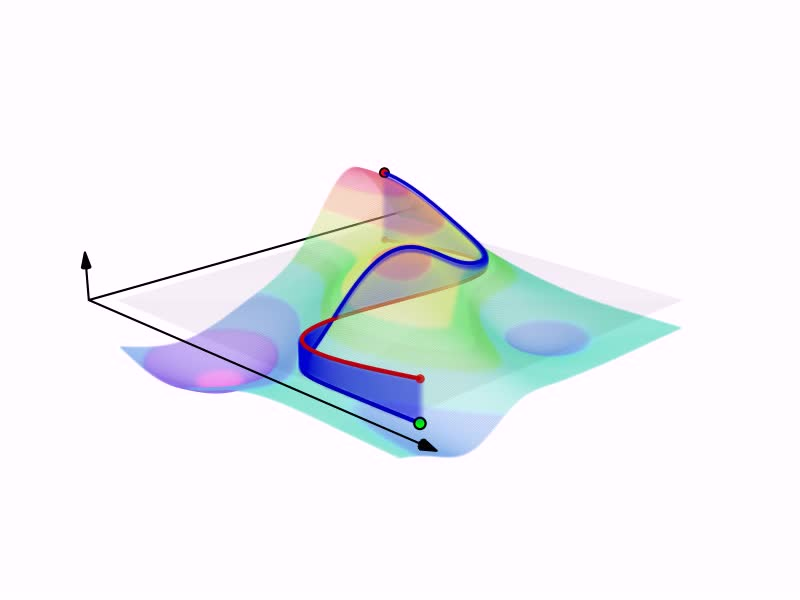
\includegraphics[width=.5\textwidth]{Figures_Part_6/Line_integral_of_scalar_field.jpg}
                       \end{figure}
                       
                       \begin{ex}{Length of a curve}{length_of_curve}
                       Let $f(x,y,z)=1$ and $\curvegamma(t)$ be a curve over $t=a$ to $t=b$.  Then the line integral
                       \[
                       \int_{\curvegamma} fd\curvegamma = \int_a^b \left|\tangentgamma(t)\right|dt
                       \]
                      which is the length of the curve $\curvegamma$.
                       \end{ex}
                       
                       \begin{ex}{Line Integral on a Paraboloid}{line_int_parabooid}
                       Consider the function $f(x,y)=x^2+y^2$ and $\curvegamma(t)=\begin{pmatrix} t \\ t \end{pmatrix}$ over $t=0$ to $t=1$.  Then the line integral
                       \[
                       \int_{\curvegamma} fd\curvegamma = \int_0^1 f(\curvegamma(t))\left|\tangentgamma(t)\right|dt.
                       \]
                       We have
                       \begin{itemize}
                           \item $f(\curvegamma(t))=t^2+t^2=2t^2.$
                           \item $\left|\tangentgamma(t)\right|=\left|\begin{pmatrix} 1 \\ 1\end{pmatrix}\right|=\sqrt{2}.$
                       \end{itemize}
                       So we have
                       \[
                       \int_{\curvegamma} fd\curvegamma = \int_0^1 2\sqrt{2}t^2dt.
                       \]
                       This evaluates to $\frac{2\sqrt{2}}{3}$.
                       \end{ex}
                       
                       \begin{exercise}
                       Integrate $f(x,y)=x+y$ along the curve $\curvegamma(t)=\begin{pmatrix} t \\ 0 \end{pmatrix}$ from $t=0$ to $t=1$. What do you notice about this? Can we tie this to one-dimensional integration?
                       \end{exercise}
                       
                                	        
                   	